\chapter{Experimental setup}

\intro{The measurements within this thesis are based on proton-proton collision data recorded with the CMS detector in 2012, 2015, and 2016 at center-of-mass energies of 8 and 13~\TeV. The experimental setup is described in this chapter. First, the \gls{lhc}~\cite{Evans:2008zzb}, its preacceleator chain and other experiments at the \gls{lhc} are briefly introduced. Then the CMS detector and its components are detailed. A review of the operations summarizes the chapter.}

%##############################################
\section{Large Hadron Collider}
%##############################################

The \glsreset{lhc}\gls{lhc} is a 26.7~km long accelerator and storage ring for protons and heavy ions at the \glsreset{cern}\gls{cern}, Geneva, Switzerland. It was constructed between 1998\range2008 in the existing tunnel of the former \glsreset{lep}\gls{lep} which lies 45\range170~m below the surface. The \gls{lhc} ring features two beam pipes which can be separately filled with up to 2'808 countercycling bunches of protons with a bunch-to-bunch spacing of 25~ns per pipe. The beams can be focused for collision at four \glspl{ip}. The design allows to accelerate protons with a momentum of 450~\GeV at injection to up to 7~\TeV yielding a center-of-mass energy of 14~\TeV in collisions.

To bend the beams 1'232 dipol cryostats are deployed hosting both beam pipes and two dipol magnets within a cold mass in a twin-bore design. The cold mass itself is placed in a vacuum vessel for thermal insulation. The magnet coils consist of \gls{nbti} alloy fibers which are cooled down to 1.9~K using superfluid helium. At this temperature, the magnets are superconducting. This allows to produce the required magnetic field strength to sustain a closed beam orbit ranging from 0.54~T at injection energy to up to 8.33~T for the maximum beam energy. At maximum field a current of 11850~A is required. Such high magnetic fields cannot be achieved with normal conductors due to magnetic saturation. 

Additional about 3'800 single aperture and 1'000 twin aperture magnets are installed to keep the beam particles focused around the nominal orbit~(quadrupoles) and for further orbit corrections~(sextu-, octu-, and decapoles). Special quadrupole triplets at each side of the four \glspl{ip} focus the beams for collision. The envelop of the particle trajectories with respect to the nominal beam orbit is described by the beta function which can be approximated around the \glspl{ip} as 

\begin{equation}
\beta(x)=\beta^\star+\frac{x^2}{\beta^\star}.
\end{equation}

At two high luminosity \glspl{ip}, the beams can be squeezed to $\beta^\star=0.55~\mathrm{m}$.\todo{performance was much better} The transverse beam size is given as $\sigma^{\star}=\sqrt{\epsilon_\mathrm{n}\cdot\beta^\star/\gamma}\approx17~{\mu\mathrm{m}}$ for $\gamma=E/m_\mathrm{p}\approx7000$ where $\epsilon_\mathrm{n}$ denotes the normalized beam emittance. It is a measure of the phase space area occupied by the particles within the beam which is constant following Liouville's theorem. The emittance cannot be larger than $\epsilon_\mathrm{n}>3.75~\mu\mathrm{m}\cdot\mathrm{rad}$ in order to not loose significant amounts of the beam in the \gls{lhc} arcs where $\beta(x)$ is the largest.

The expected luminosity at the \glspl{ip} can be calculated from the machine and beam parameters as

\begin{equation}
L=\frac{N_\mathrm{p}^{2}n_\mathrm{b}f\gamma}{4\pi\sigma^{2}}\cdot F
\end{equation}

where $N_\mathrm{p}$ denotes the number of protons per bunch, $n_\mathrm{b}$ the number of colliding bunches, and $f$ the beam revolution frequency. The factor 

\begin{equation}
F=1\Bigg/\sqrt{1+\Big(\frac{\theta\cdot\sigma_{z}}{2\sigma^\star}\Big)^2}
\end{equation}

accounts for a reduction in luminosity due to the crossing angle $\theta$ of the beams. frequency, np,->lumi

Lumi, pileup





 yielding a magnetic field of 

 that is accommodate both beam pipes in a common twin-bore design.



A gap of ? allows to ramp up kicker magnets for injection or beam dump.




The \gls{lhc} ring consists of eight straight and eight curved sections. 

Two transfer tunnels connect the \gls{lhc} to the accelerator complex at \gls{cern}.

beta, emittance, lumi, beam profile, pipe vaccum, collimator, cavities, beam dump, monitoring, scrubbing, quench training, energy measurement

More information on the \gls{lhc} can be found in Ref.~\cite{Evans:2008zzb}.

%##############################################
\subsection{Accelerator complex}
%##############################################

\myfigure{The accelerator complex at CERN. The figure is taken in parts from Ref.~\cite{Mobs:2225847}.}{
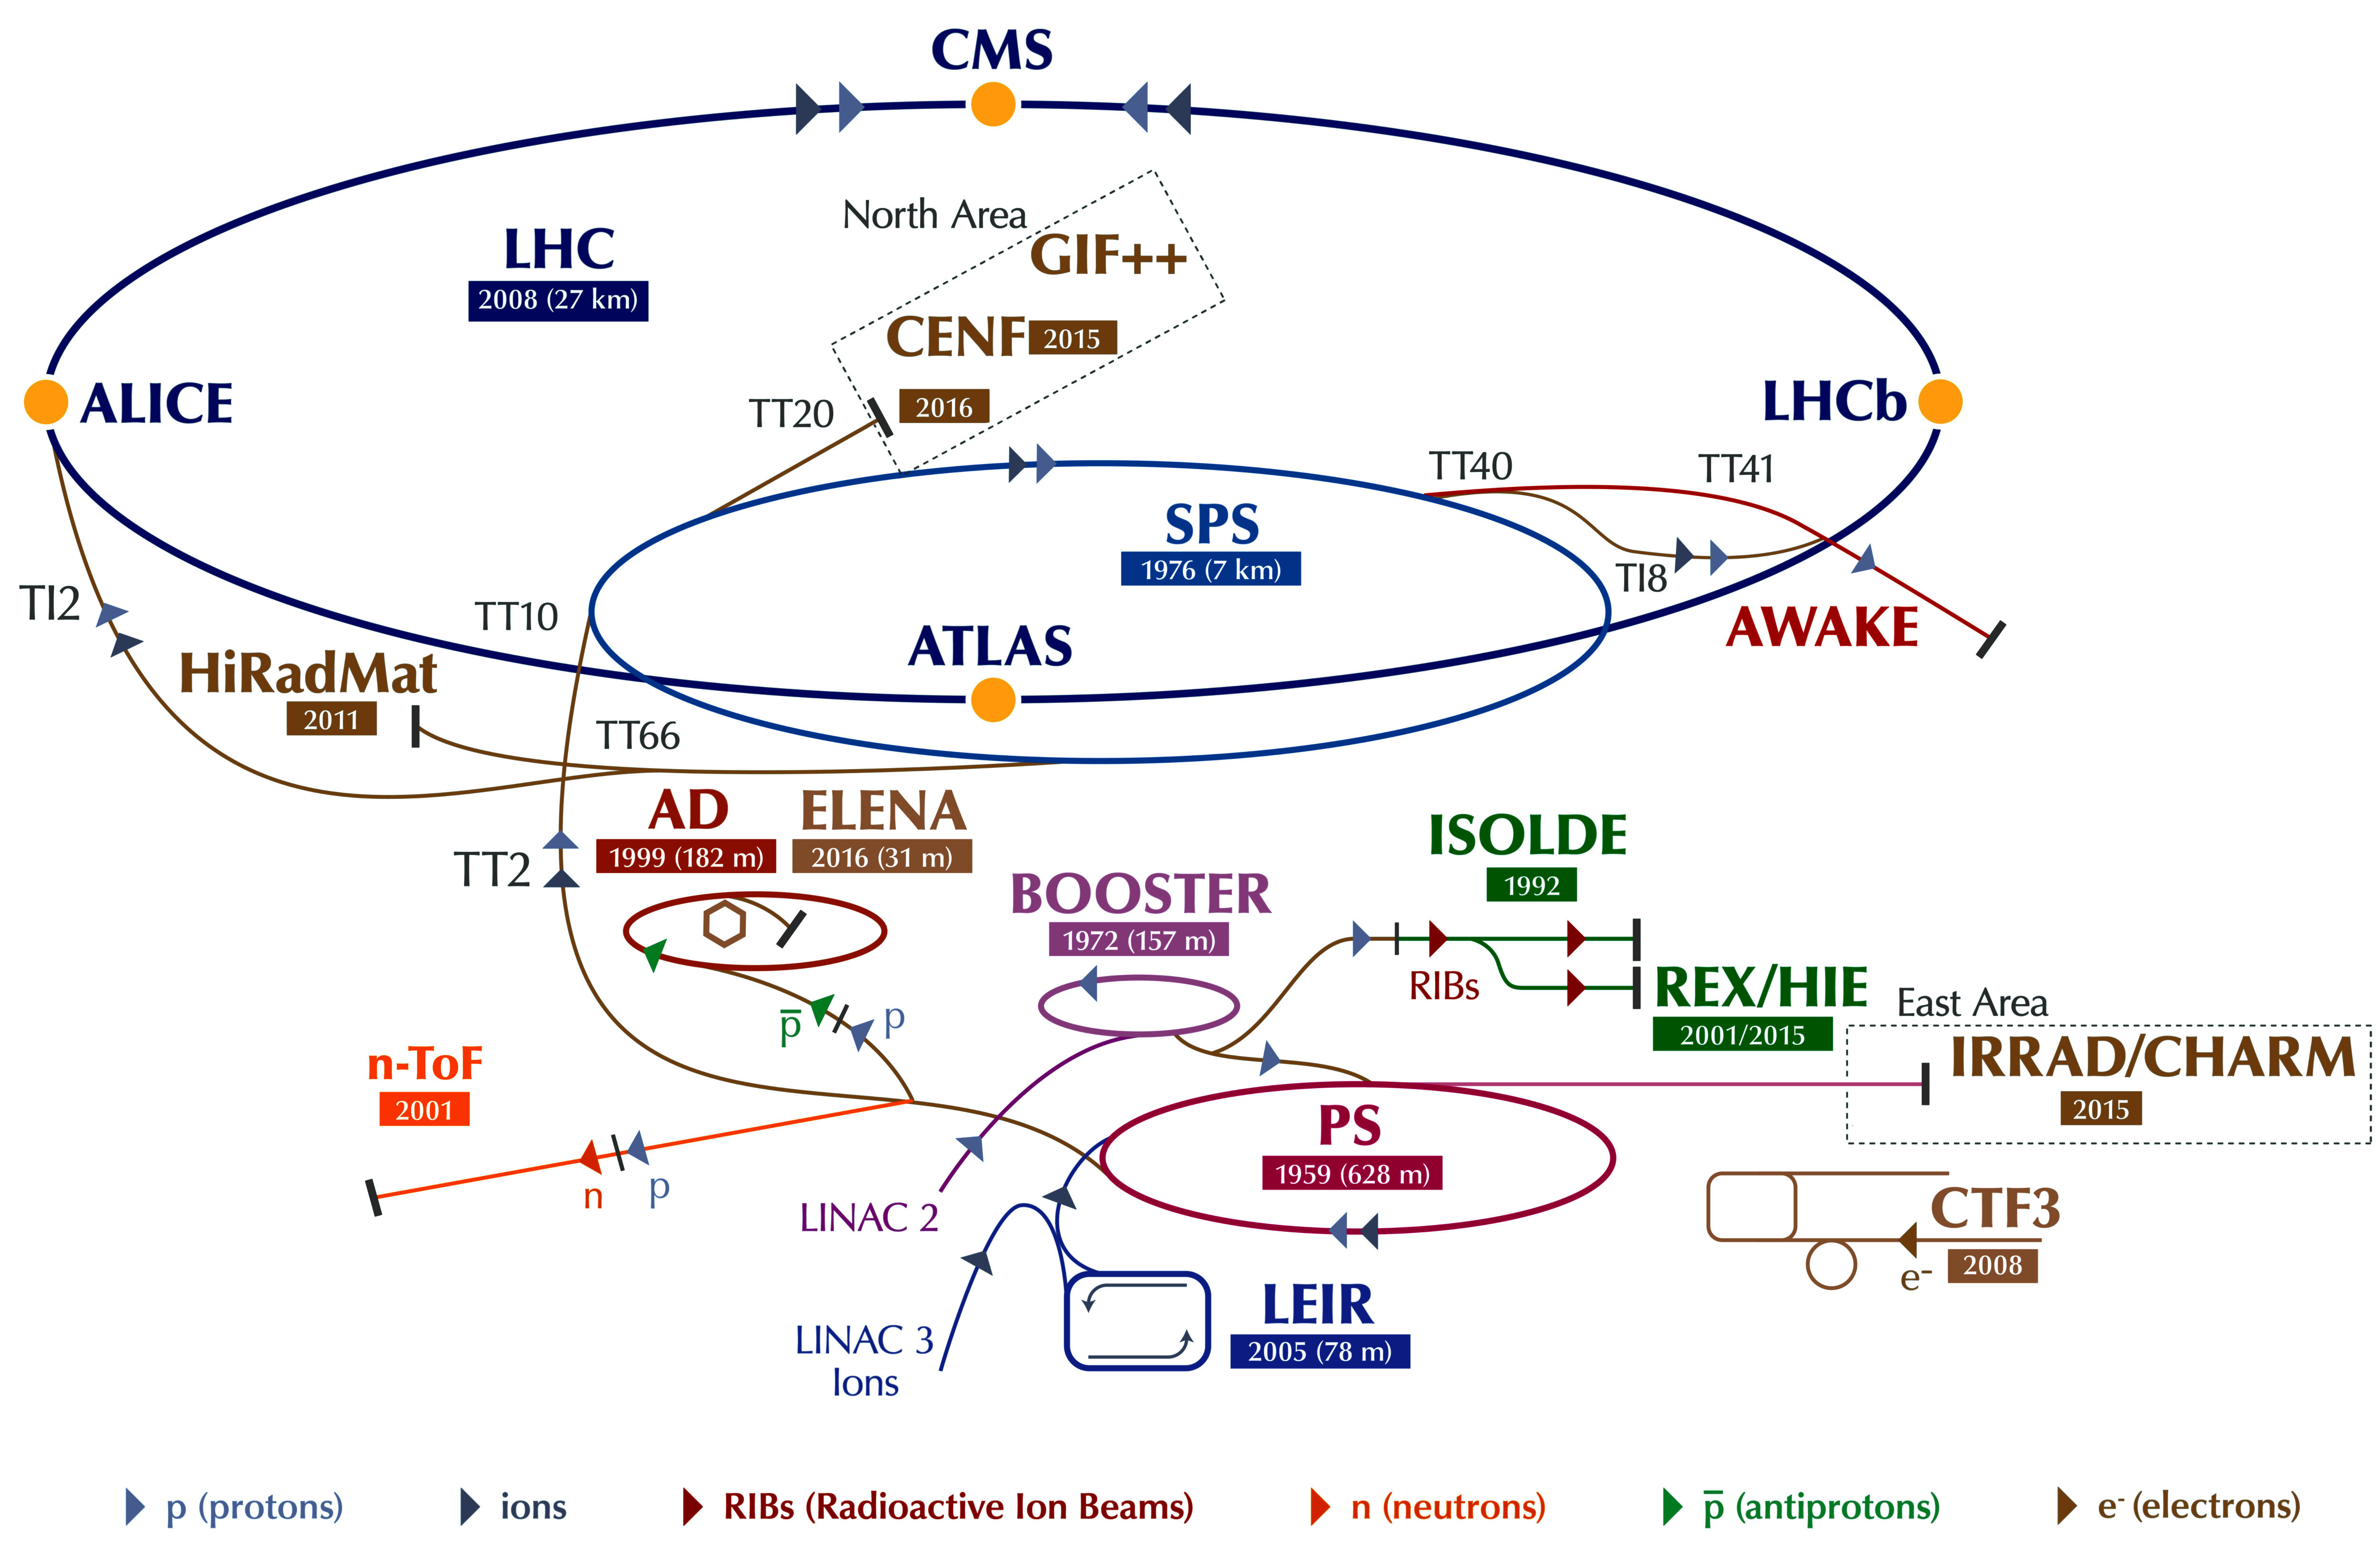
\includegraphics[width=0.99\textwidth]{figures/experiment/CERN_accelerator_complex.jpg}
}



momentum compaction

%##############################################
\subsection{Experiments}
%##############################################

%##############################################
\section{CMS experiment}
%##############################################

\myfigure{The figure is taken in parts from Ref.~\cite{Bayatian:2006zz}.}{
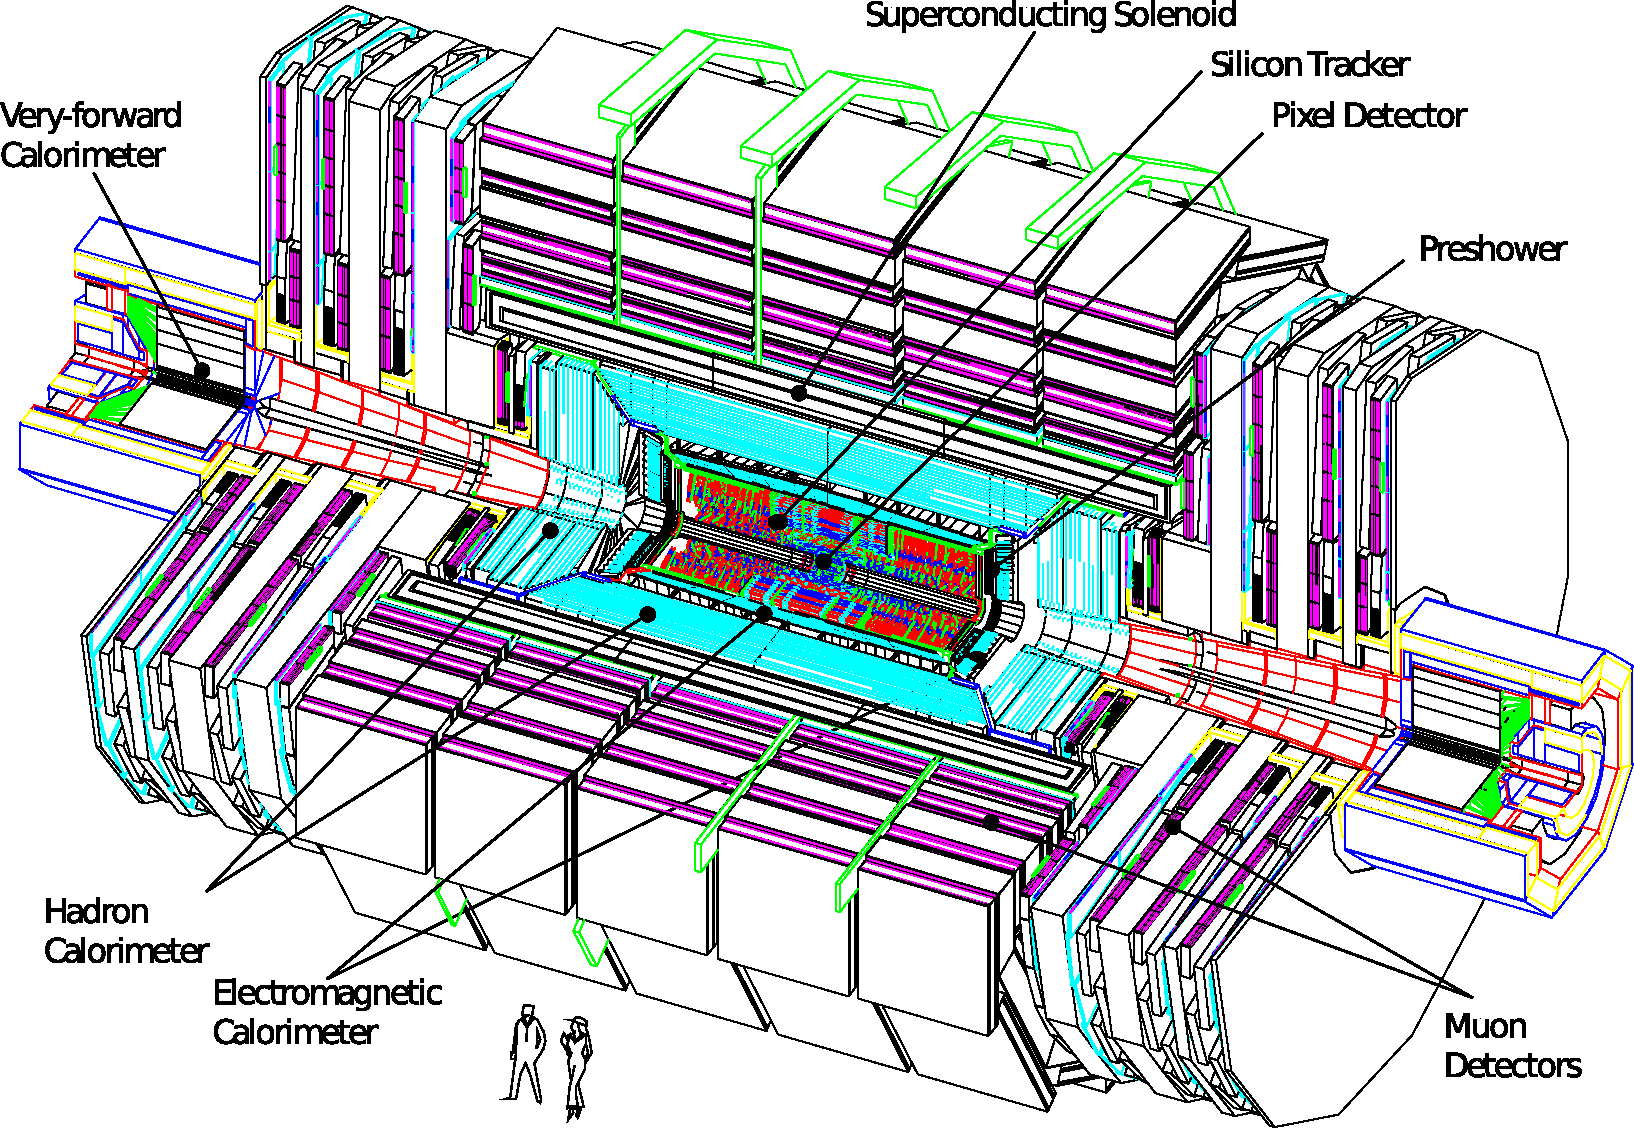
\includegraphics[width=0.99\textwidth]{figures/experiment/CMS_overview.pdf}
}

%##############################################
\subsection{Magnet}
%##############################################

\cite{Acquistapace:1997fm}

%##############################################
\subsection{Tracker}
%##############################################



\cite{Chatrchyan:2014fea}

%##############################################
\subsection{Electromagnetic calorimeter}
%##############################################

%##############################################
\subsection{Hadronic calorimeter}
%##############################################

%##############################################
\subsection{Muon systems}
%##############################################
DT/RPC/CSC

%##############################################
\subsection{Data acquisition}
%##############################################
Trigger/DAQ

%##############################################
\subsection{Operations}
%##############################################
DCS/DSS
